%
%~~
%~~ Objective-C e classe Cocoa Touch
%~~
%

\chapter{\emph{Objective-C} e \emph{Cocoa Touch}} % (fold)
\label{cha:objective_c_e_classe_cocoa_touch}

\emph{Objetive-C} � a linguagem prim�ria usada para construir \emph{softwares} para macOS e iOS baseada na linguagem C, com programa��o orientada a objeto. A origem dos conceitos s�o relacionados � linguagem \emph{Smalltalk}, uma das primeiras linguagens orientada a objeto.

\emph{Cocoa Touch} � um \emph{framework} de padr�o de projeto utilizado no iOS com foco espec�fico na interface orientada a toques. Fornece ferramentas b�sicas para implementar, como por exemplo o \emph{UIKit} que � o respons�vel pelo visual das aplica��es do sistema operacional, como tamb�m gerenciamento de dados na aplica��o, conex�o, constru��o de \emph{strings}, aceler�metro, etc.

Para caracter�sticas mais espec�ficas da aplica��o � separada a parte em outros pacotes de desenvolvimento dentro do \emph{Cocoa Touch}. Alguns exemplos:
\begin{enumerate}
	\item \emph{Core Animation}
	\item \emph{Core Data}
	\item \emph{Core Audio}
	\item \emph{Core}
\end{enumerate}

Tamb�m tem como base o \emph{Core OS} e o \emph{Core Services}, utilizados no \emph{MacOS}.


\begin{figure}
	\centering
	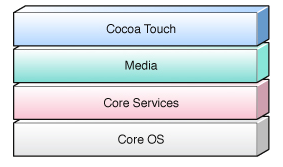
\includegraphics[scale=0.8]{img/iphone/CocoaTouch.png}
	\caption{Camadas base do \emph{Cocoa Touch}}
\end{figure}



% chapter objective_c_e_classe_cocoa_touch (end)